%****************************************************************
% Chapter X
%****************************************************************
\label{chapter-performance}
\chapter{Performance}

%****************************************************************
What is great about the Android runtime is that most of the stress of memory reclamation is done for developers. The system will track what developers are doing and when it sees that an object is not needed anymore, it will free it on their behalf. However, this does not exclude performance problems from happening here. When the amount of memory have allocated reaches an upper limit, a Garbage Collection (GC) event will be kicked off to free any resources that might not be needed any longer, freeing up space for future allocations. 

Anytime the frame drips about the $16$ milliseconds barrier, and the users are going to start to notice. Therefore, any code that forces allocated memory to spike above this threshold can cause problems. For instance, memory can become tighter, if the developer is allocating and freeing a large number of objects in a short period of time, the temporary objects again kicking off GC event. 

\begin{figure}[H]
\caption{16ms Per Frame}
\label{fig:16ms-per-frame}
\centering
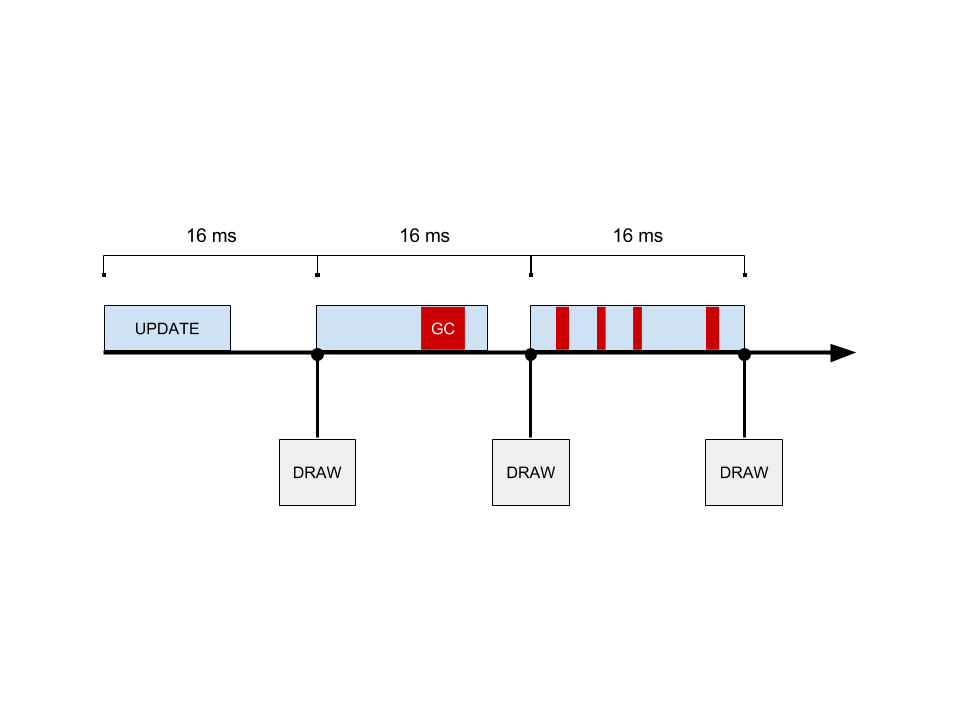
\includegraphics[width=\textwidth, keepaspectratio]{Figures/16ms-per-frame.png}
\decoRule
\end{figure}

Therefore, a performance testing is important for avoiding nasty GC events. Each GC event that developer can avoid, the application has more time per frame to do interesting things. In order to find out where in the code objects are being created but not released, created and not used, or created new when the developer could have been reusing them from existing objects. Android Studio provides a series of performance testing tools, such as Memory Monitor, Allocation Tracker, Heap Viewer, and the Systrace (it is an Android system trace tool helps developers analyze how the execution of the application fits into the many running systems on an Android device \cite{google.systrace.2016}). According to the runtime, the performance analysis is divided into two parts: acyclic process and cyclic process (performance data came from Android phone $Nexus 6P$.).

%****************************************************************
\section{Acyclic}

%****************************************************************
In order to avoid UI being block, all of acyclic process in the application are handled in the new threads. In this section, I present the performance of geometric vertices' generation for \code{Placemark} (Icosphere) and \code{Earth} (UV Sphere) which only executes one time (or not) when needed. The geometric data from Icosphere generation will be cached once it has been created. This is useful to avoid duplicate creations for same geometric vertices. In the \code{Placemark} description URL analysis, the same cache solution for image and text.

%****************************************************************
\subsection{Icosphere Generator}

%****************************************************************
Based on the varying roundness of the Icosphere, it could evolve into a sphere has different vertex count \ref{tab:icosphere-level}. In general, level $3$ Icosphere is enough for illustrating a sphere, and in the application the \code{Placemark} is created on level $1$ Icosphere.

\begin{table}[H]
	\caption{Icosphere Level}
	\label{tab:icosphere-level}
	\centering
	\begin{tabular}{l l}
		\toprule
		\tabhead{Recursion Level} & \tabhead{Vertex Count}\\
		\midrule
		0 & 12\\
		1 & 42\\
		2 & 162\\
		3 & 642\\
		4 & 2562\\
		5 & 10242\\
		\bottomrule
	\end{tabular}
\end{table}

\begin{figure}[H]
	\caption{Icosphere performance}
	\label{fig:icosphere-performance}
	\centering
	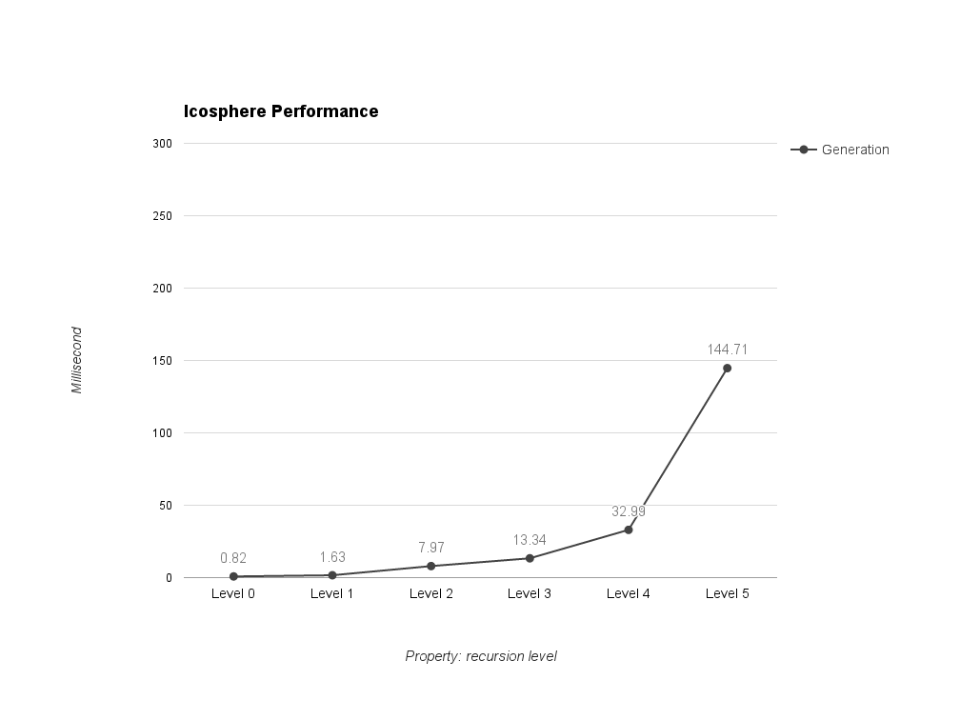
\includegraphics[width=\textwidth, keepaspectratio]{Figures/icosphere-performance.png}
	\decoRule
\end{figure}

%****************************************************************
\subsection{UV Sphere Generator}

%****************************************************************
The roundness of a UV Sphere depends on the partition level on both horizontal (ring) and vertical (segment) which denotes the axes of the 2D texture. The Earth is casually implemented as a $180 / 180$ UV Sphere in the application.

\begin{figure}[H]
	\caption{UV Sphere performance}
	\label{fig:uv-sphere-performance}
	\centering
	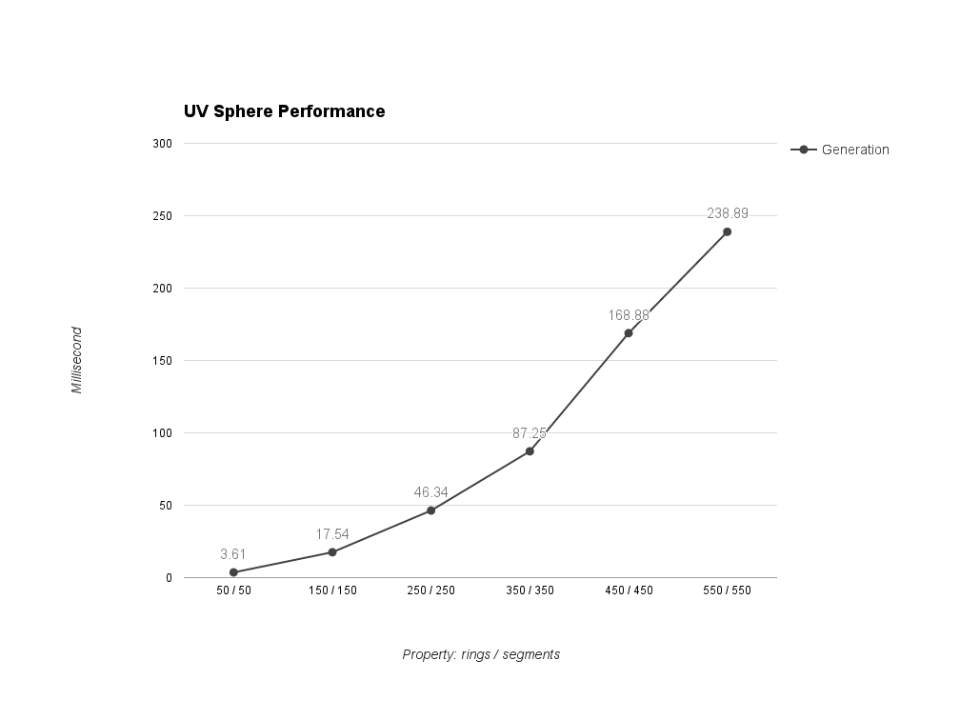
\includegraphics[width=\textwidth, keepaspectratio]{Figures/uv-sphere-performance.png}
	\decoRule
\end{figure}

%****************************************************************
\subsection{Geographic Data Initialization}

%****************************************************************
Figure \ref{fig:geographic-data-performance} is the performance of initializing geographic data, including parsing KML files, transformation coordinate system from LLA to ECEF for each \code{Placemark}, etc.

\begin{figure}[H]
	\caption{Geographic Data Performance}
	\label{fig:geographic-data-performance}
	\centering
	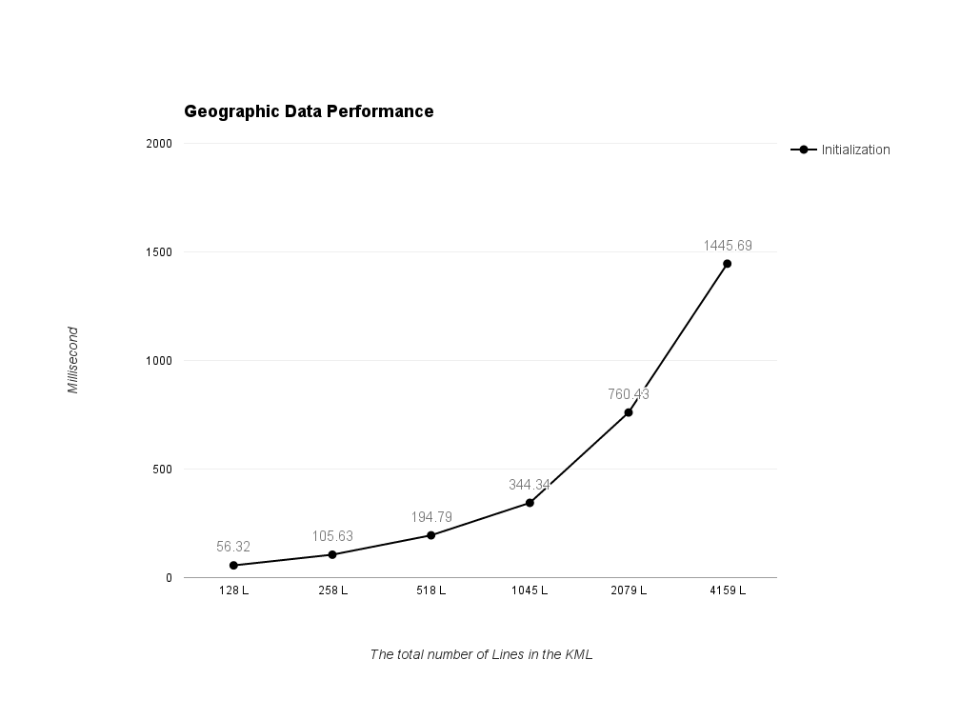
\includegraphics[width=\textwidth, keepaspectratio]{Figures/geographic-data-performance.png}
	\decoRule
\end{figure}

%****************************************************************
\section{Cyclic}

%****************************************************************
Task that required repeatedly executed during the rendering cyclicity of each frame is the factors influencing the runtime performance. They are ray-model intersection detection, update models, and draw models. In this section, I present the result of memory leak analysis and crucial tasks that closely related to performance.

%****************************************************************
\subsection{Memory Leak}

%****************************************************************
I am using Memory Monitor to evaluate memory leak. As the application allocates and free memory, we will see the allocative amount fluctuate in the graph at the same time. Any time the allocated memory drops by a significant amount, that is a signal that GC event has occurred (see \ref{fig:memory-monitor}). These GC events are not generally a noticeable performance problem, however a lots of them occurring over and over and over again in a short period of time can actually lead to performance issues. Additionally, it more or less created memory leaks, which are objects which the application is no longer using, but the garbage collector fails to recognize them as unused.

\begin{figure}[H]
	\caption{Memory Monitor \cite{google.memory-monitor.2015}}
	\label{fig:memory-monitor}
	\centering
	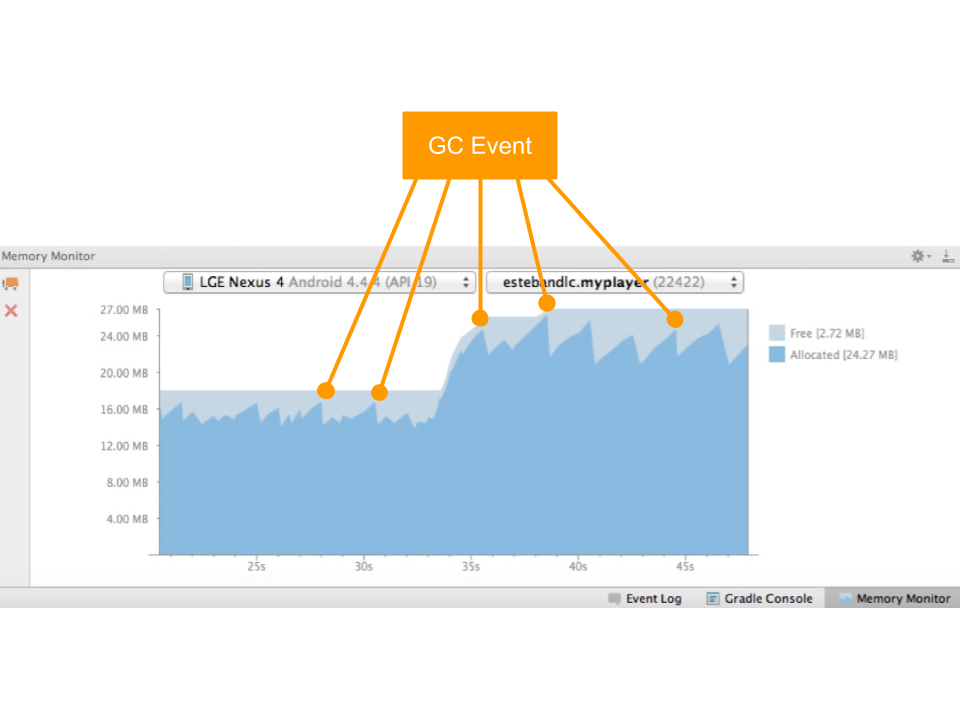
\includegraphics[width=\textwidth, keepaspectratio]{Figures/memory-monitor.png}
	\decoRule
\end{figure}

In a world where your application is not doing much of anything, you should see a flat graph. From a performance perspective, this is actually an ideal scenario. The more time you are spending doing GC, the less time you will have to do other stuff. Fortunately, with a careful in dealing with objects, I got a quite flat runtime memory allocation graph \ref{fig:memory-performance}.

\begin{figure}[H]
	\caption{Memory Performance}
	\label{fig:memory-performance}
	\centering
	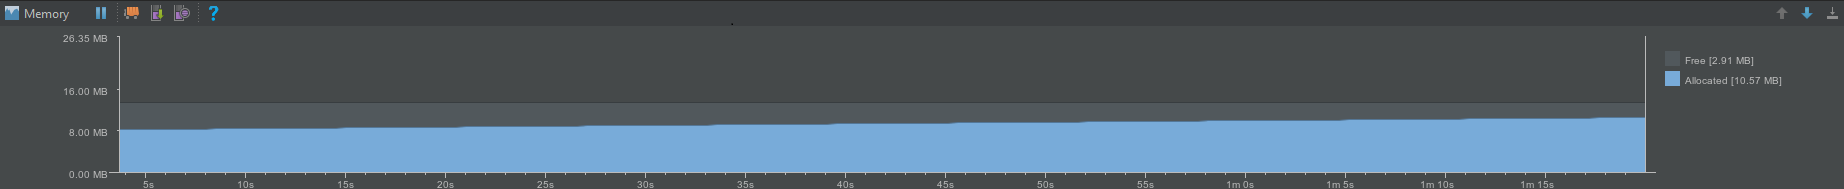
\includegraphics[width=\textwidth, keepaspectratio]{Figures/memory-performance.png}
	\decoRule
\end{figure}

%****************************************************************
\subsection{Placemarks Intersection}

%****************************************************************



\begin{figure}[H]
	\caption{Placemarks Intersection Performance}
	\label{fig:placemarks-intersection-performance}
	\centering
	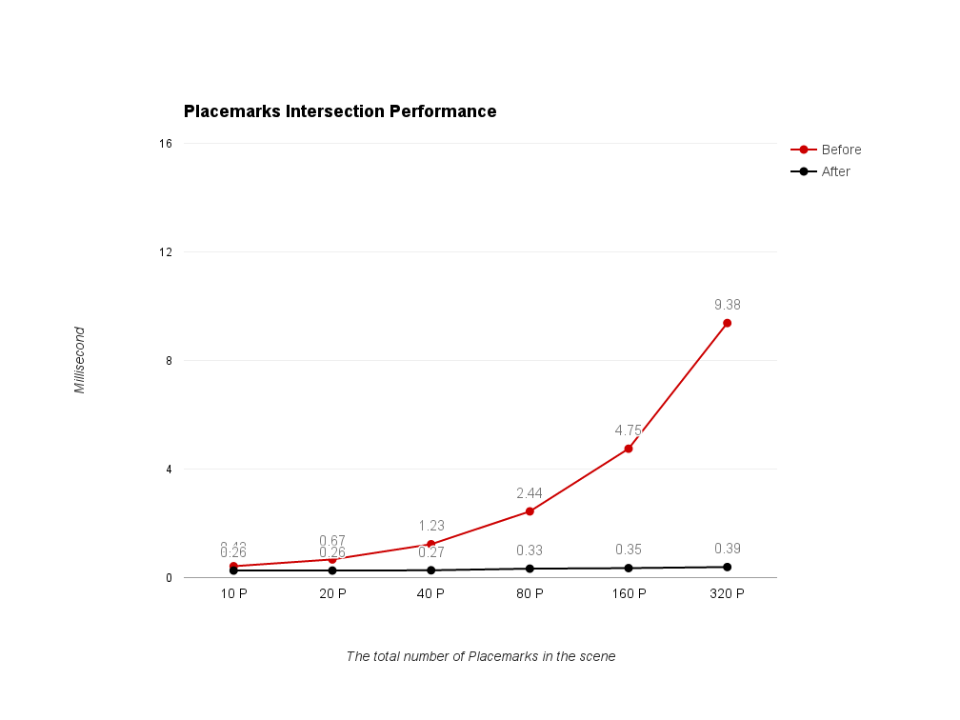
\includegraphics[width=\textwidth, keepaspectratio]{Figures/placemarks-intersection-performance.png}
	\decoRule
\end{figure}



%****************************************************************
\subsection{Placemarks Update}
\label{section:placemarks-update}

%****************************************************************



\begin{figure}[H]
	\caption{Placemarks Update Performance}
	\label{fig:placemarks-update-performance}
	\centering
	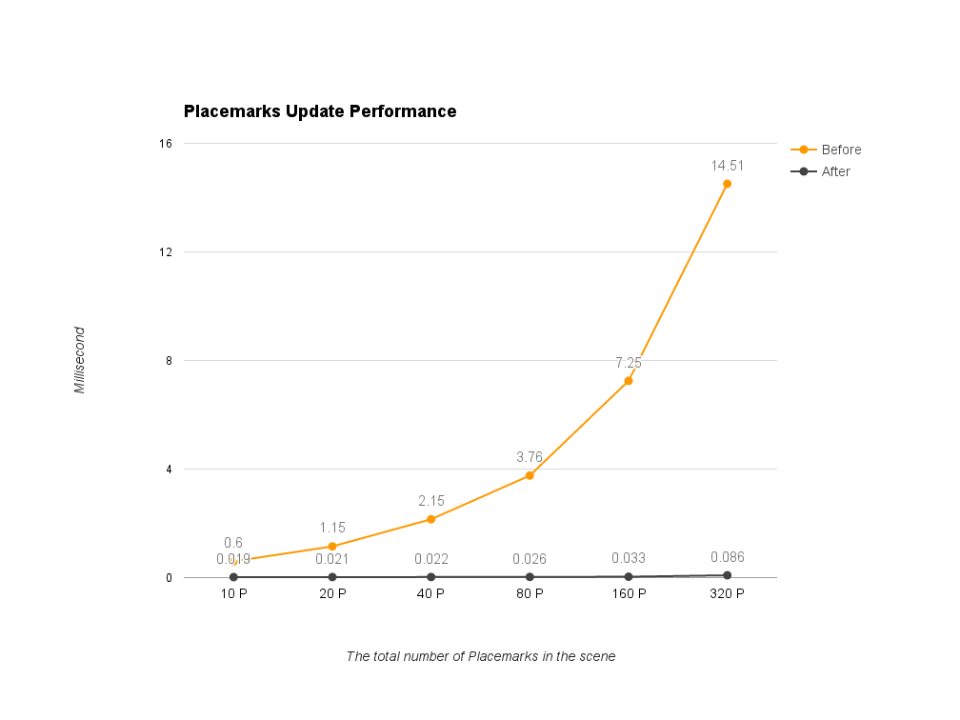
\includegraphics[width=\textwidth, keepaspectratio]{Figures/placemarks-update-performance.png}
	\decoRule
\end{figure}



%****************************************************************
\subsection{Placemarks Draw}

%****************************************************************



\begin{figure}[H]
	\caption{Placemarks Draw Performance}
	\label{fig:placemarks-draw-performance}
	\centering
	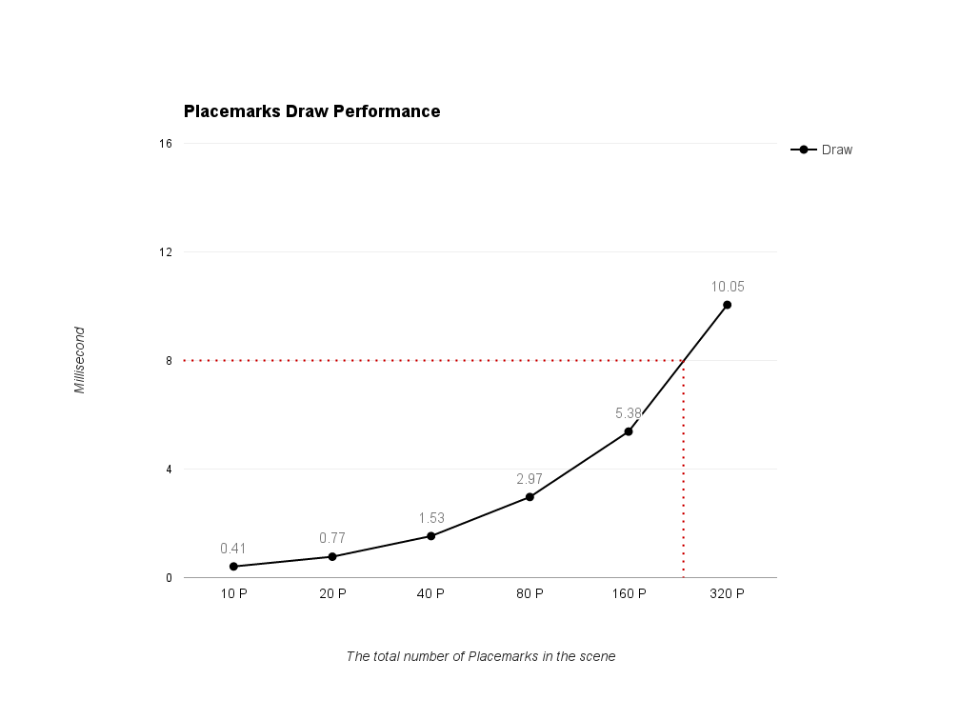
\includegraphics[width=\textwidth, keepaspectratio]{Figures/placemarks-draw-performance.png}
	\decoRule
\end{figure}



\begin{figure}[H]
	\caption{glDrawElements Performance}
	\label{fig:glDrawElements-performance}
	\centering
	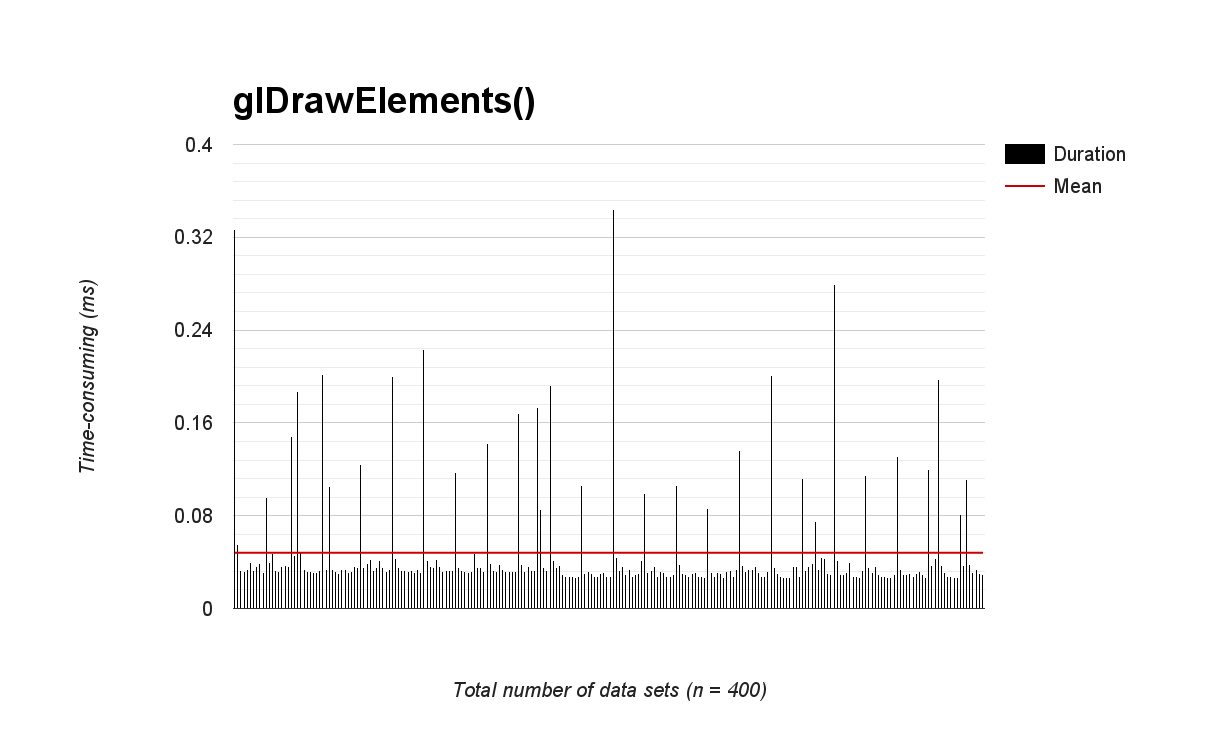
\includegraphics[width=\textwidth, keepaspectratio]{Figures/glDrawElements-performance.png}
	\decoRule
\end{figure}



%****************************************************************